\section{Modelo conceptual del Caso de Uso}

\subsection{Descripción general}
En la figura~\ref{fig:conceptualProyectos} se muestra la estructura de información de los elementos que componen un caso de uso.
 
\begin{figure}[htbp!]
	\begin{center}
		\fbox{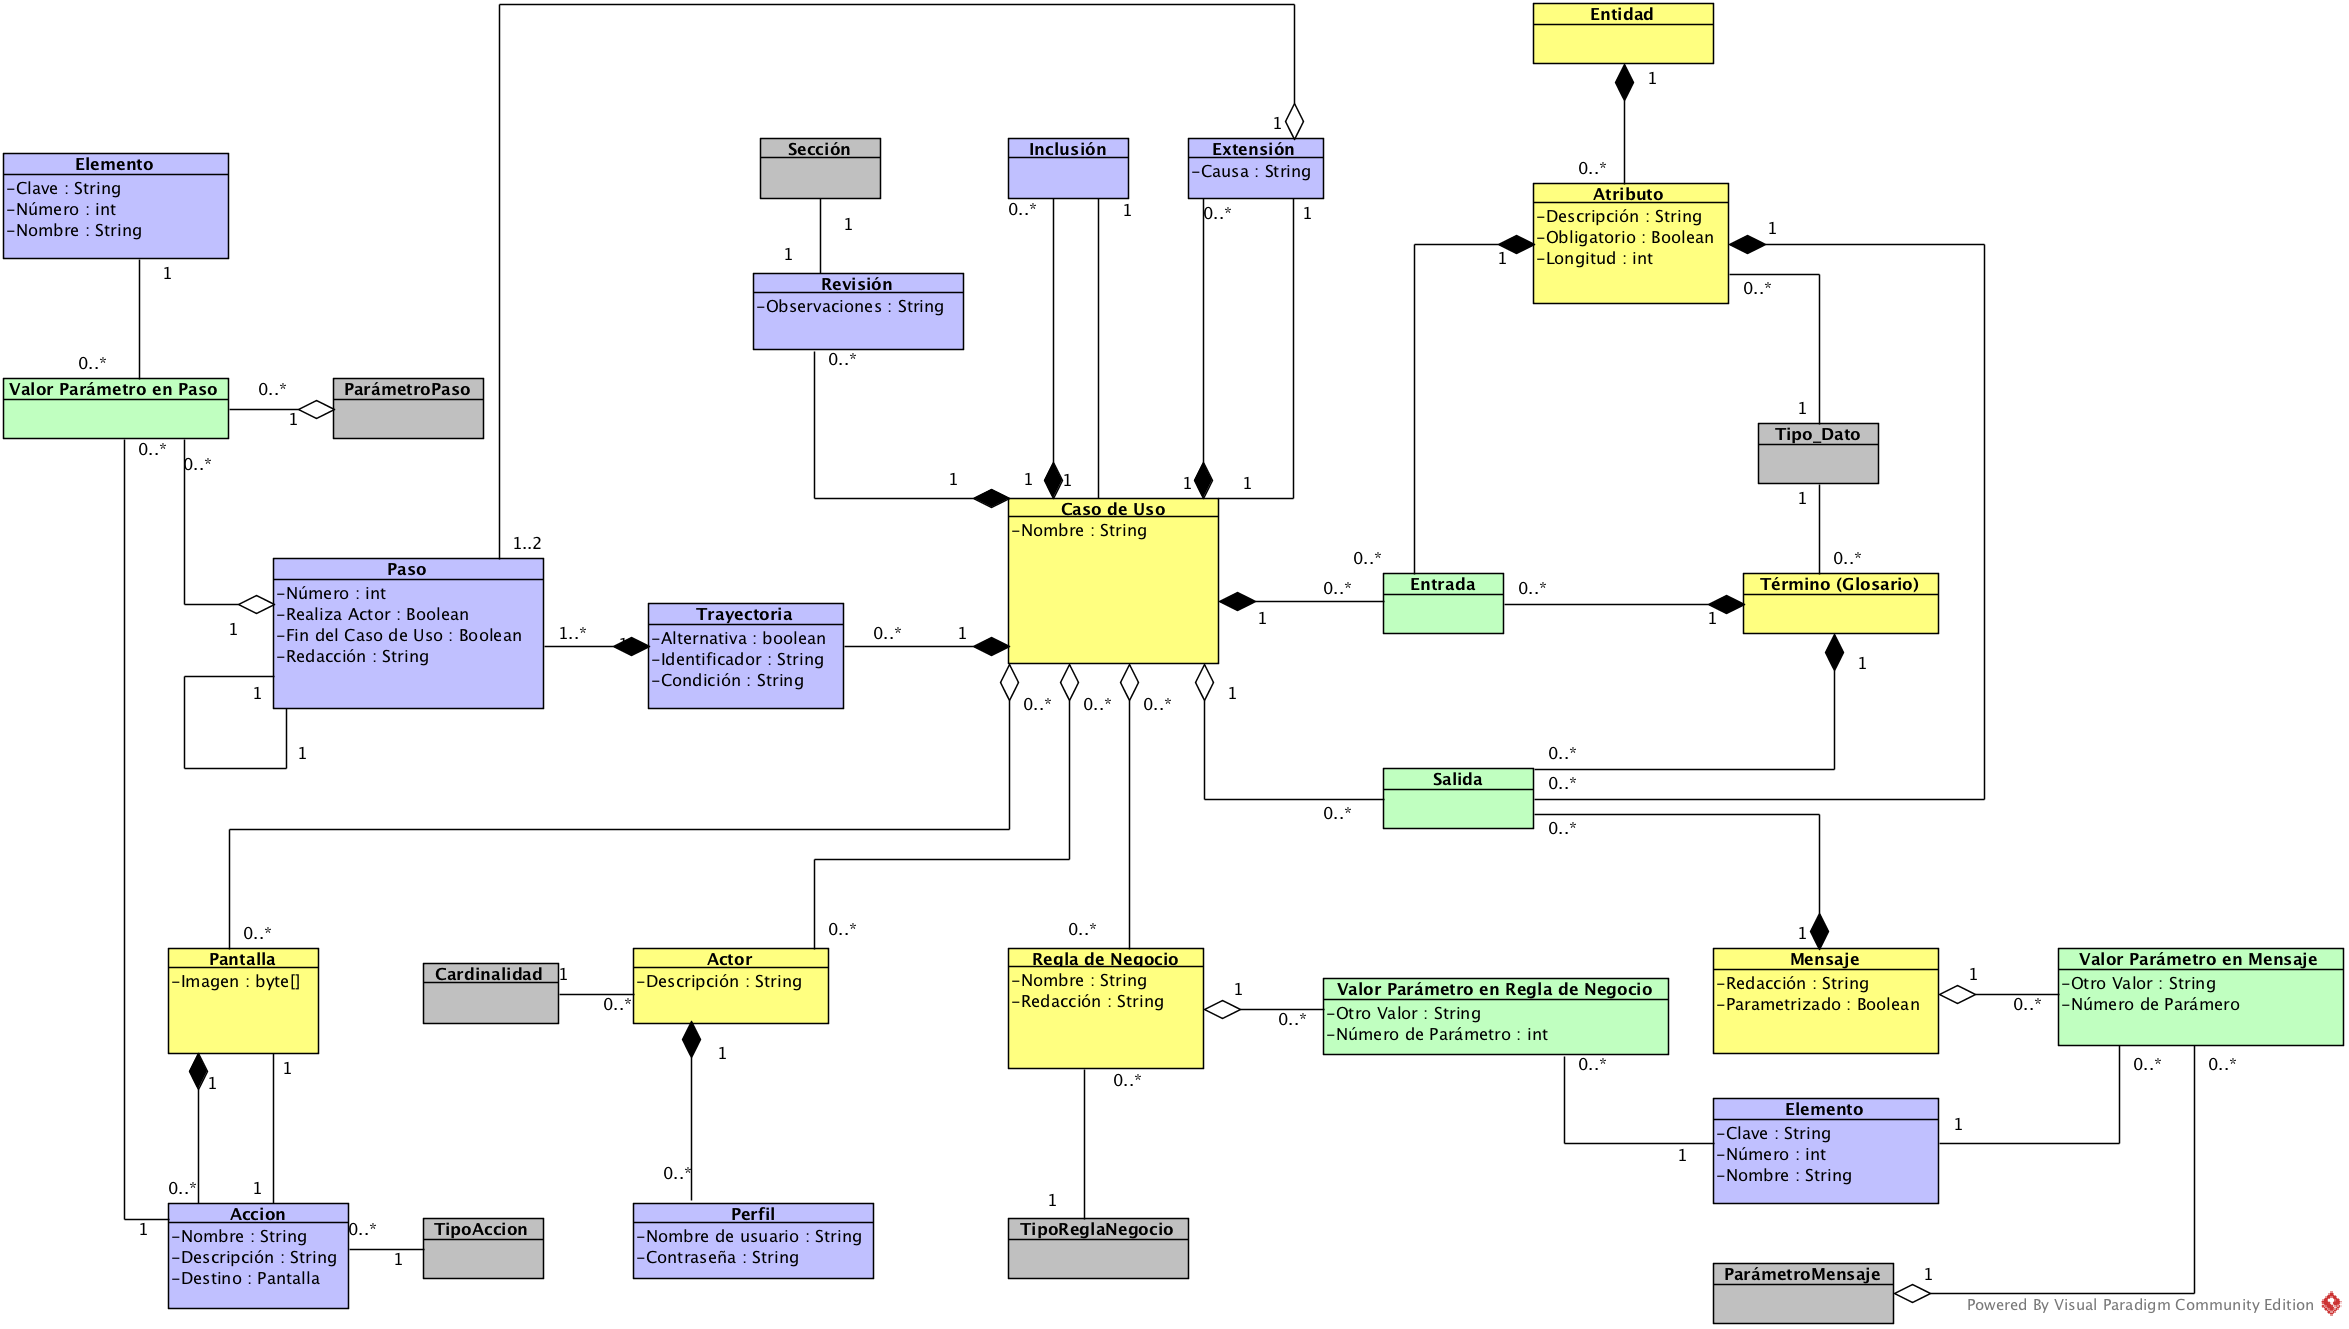
\includegraphics[width=1\textwidth]{ModeloNegocios/images/ModeloConceptualCasoUso}}
		\caption{Modelo conceptual de casos de uso}
		\label{fig:conceptualProyectos}
	\end{center}
\end{figure}


%-------------------------------------------------Caso de Uso----------------------------------

\begin{BusinessEntity}{CasodeUso}{Caso de Uso}
      \Battr{Clave}{Clave}{\tdPalabra}{Clave que permitirá distinguir el que el Elemento es un Caso de Uso}{\requerido}
      \Battr{Numero}{Número}{\tdNumerico{entero}}{Número del Caso de Uso}{\requerido}
      \Battr{Nombre}{Nombre}{\tdFrase}{Nombre que identificará al Caso de Uso}{\requerido}
\end{BusinessEntity}

\subsubsection{Relaciones}

\begin{BusinessFact}{CasodeUso:Pantalla}{Pantalla}
	\BRitem{Descripción}{Un Caso de Uso utiliza diferentes pantallas.}
	\BRitem{Tipo}{\relAgregacion}
    \BRitem{Cardinalidad}{Muchos a muchos}
	
\end{BusinessFact}

\begin{BusinessFact}{CasodeUso:Actor}{Actor}
	\BRitem{Descripción}{Un Caso de Uso puede ser realizado por diferentes actores.}
	\BRitem{Tipo}{\relAgregacion}
    \BRitem{Cardinalidad}{Muchos a muchos}
\end{BusinessFact}

\begin{BusinessFact}{CasodeUso:ReglaNegocio}{Regla de Negocio}
	\BRitem{Descripción}{Un Caso de Uso puede utilizar diferentes relgas de negocio.}
	\BRitem{Tipo}{\relAgregacion}
    \BRitem{Cardinalidad}{Muchos a muchos}
	
\end{BusinessFact}

\begin{BusinessFact}{CasodeUso:Salida}{Salida}
	\BRitem{Descripción}{Un caso de uso tiene diferentes salidas.}
	\BRitem{Tipo}{\relComposicion}
    \BRitem{Cardinalidad}{Uno a muchos}
\end{BusinessFact}

\begin{BusinessFact}{CasodeUso:Entrada}{Entrada}
	\BRitem{Descripción}{Un caso de uso tiene diferentes entradas.}
	\BRitem{Tipo}{\relComposicion}
    \BRitem{Cardinalidad}{Uno a muchos}
\end{BusinessFact}

\begin{BusinessFact}{CasodeUso:Trayectoria}{Trayectoria}
	\BRitem{Descripción}{Un caso de uso se compone de trayectorias.}
	\BRitem{Tipo}{\relComposicion}
    \BRitem{Cardinalidad}{Uno a muchos}
\end{BusinessFact}

\begin{BusinessFact}{CasodeUso:Revision}{Revision}
	\BRitem{Descripción}{Un caso de uso puede ser revisado.}
	\BRitem{Tipo}{\relComposicion}
    \BRitem{Cardinalidad}{Uno a muchos}
\end{BusinessFact}

\begin{BusinessFact}{CasodeUso:Extension}{Extension}
	\BRitem{Descripción}{Un caso de uso puede tener puntos de extensión.}
	\BRitem{Tipo}{\relComposicion}
    \BRitem{Cardinalidad}{Uno a muchos}
\end{BusinessFact}

\begin{BusinessFact}{CasodeUso:Inclusion}{Inclusion}
	\BRitem{Descripción}{Un caso de uso puede incluir otros casos de uso.}
	\BRitem{Tipo}{\relComposicion}
    \BRitem{Cardinalidad}{Uno a muchos}
\end{BusinessFact}

\begin{BusinessFact}{CasodeUso:Precondicion}{Precondicion}
	\BRitem{Descripción}{Un caso de uso puede tener diferentes precondiciones.}
	\BRitem{Tipo}{\relComposicion}
    \BRitem{Cardinalidad}{Uno a muchos}
\end{BusinessFact}

\begin{BusinessFact}{CasodeUso:Postcondicion}{Postcondicion}
	\BRitem{Descripción}{Un caso de uso puede tener diferentes postcondiciones.}
	\BRitem{Tipo}{\relComposicion}
    \BRitem{Cardinalidad}{Uno a muchos}
\end{BusinessFact}

%-------------------------------------------------Pantalla----------------------------------

\begin{BusinessEntity}{Pantalla}{Pantalla}
      \Battr{Clave}{Clave}{\tdPalabra}{Clave que permitirá distinguir que el Elemento es una Pantalla}{\requerido}
      \Battr{Numero}{Número}{\tdNumerico{entero}}{Número de la Pantalla}{\requerido}
      \Battr{Nombre}{Nombre}{\tdFrase}{Nombre que identificará a la Pantalla}{\requerido}
	  \Battr{Imagen}{Imagen}{Imagen que ilustrará la interfaz gráfica del sistema.}{Es un archivo en formato PNG o JPG}{\requerido}
\end{BusinessEntity}

\subsubsection{Relaciones}

\begin{BusinessFact}{Pantalla:Accion}{Acción}
	\BRitem{Descripción}{Una pantalla puede tener un conjunto de acciones.}
	\BRitem{Tipo}{\relComposicion}
    \BRitem{Cardinalidad}{Uno a muchos}
\end{BusinessFact}

%-------------------------------------------------Accion----------------------------------
\clearpage
\begin{BusinessEntity}{Accion}{Acción}
      \Battr{Nombre}{Nombre}{\tdFrase}{Nombre que identificará a la Acción}{\requerido}	
      \Battr{Descripcion}{Descripción}{\tdParrafo}{Texto que describirá la Acción}{\requerido}
	  \Battr{Imagen}{Imagen}{Imágen que ilustrará la interfaz gráfica del sistema.}{Es un archivo en formato PNG o JPG}{\requerido}
\end{BusinessEntity}

\subsubsection{Relaciones}

\begin{BusinessFact}{Accion:Pantalla}{Pantalla}
	\BRitem{Descripción}{Una Acción llevará a una determinada Pantalla.}
	\BRitem{Tipo}{\relAsociacion}
    \BRitem{Cardinalidad}{Uno a uno}
\end{BusinessFact}

\begin{BusinessFact}{Accion:TipodeAccion}{Tipo de Acción}
	\BRitem{Descripción}{Una Acción es de un tipo específico.}
	\BRitem{Tipo}{\relAsociacion}
    \BRitem{Cardinalidad}{Muchos a uno}
\end{BusinessFact}

%-------------------------------------------------Actor----------------------------------

\begin{BusinessEntity}{Actor}{Actor}
      \Battr{Clave}{Clave}{\tdPalabra}{Clave que permitirá distinguir que el Elemento es una Actor}{\requerido}
      \Battr{Numero}{Número}{\tdNumerico{entero}}{Número del Actor}{\requerido}
      \Battr{Nombre}{Nombre}{\tdFrase}{Nombre que identificará al Actor}{\requerido}
	  \Battr{Descripcion}{Descripción}{\tdParrafo}{Texto que describirá al Actor}{\requerido}
\end{BusinessEntity}

\subsubsection{Relaciones}

\begin{BusinessFact}{Actor:Cardinalidad}{Cardinalidad}
	\BRitem{Descripción}{Un negocio cuenta con un número definido o aproximado de algún Actor.}
	\BRitem{Tipo}{\relComposicion}
    \BRitem{Cardinalidad}{Muchos a uno}
\end{BusinessFact}

%-------------------------------------------------Regla de Negocio----------------------------------
\clearpage
\begin{BusinessEntity}{RegladeNegocio}{Regla de Negocio}
      \Battr{Clave}{Clave}{\tdPalabra}{Clave que permitirá distinguir que el Elemento es una Regla de Negocio}{\requerido}
      \Battr{Numero}{Número}{\tdNumerico{entero}}{Número de Regla de Negocio}{\requerido}
      \Battr{Nombre}{Nombre}{\tdFrase}{Nombre que identificará a la Regla de Negocio}{\requerido}
	  \Battr{Redaccion}{Redacción}{\tdParrafo}{Redacción de la Regla de Negocio}{\requerido}
\end{BusinessEntity}

\subsubsection{Relaciones}

\begin{BusinessFact}{RegladeNegocio:TipodeRegladeNegocio}{Tipo de Regla de Negocio}
	\BRitem{Descripción}{Una Regla de Negocio es de un tipo específico.}
	\BRitem{Tipo}{\relAsociacion}
    \BRitem{Cardinalidad}{Muchos a uno}
\end{BusinessFact}

\begin{BusinessFact}{RegladeNegocio:ValordelParametroenRegladeNegocio}{Valor del Parámetro en Regla de Negocio}
	\BRitem{Descripción}{Valor de los parámetros ocupados al definir la Regla de Negocio.}
	\BRitem{Tipo}{\relAgregacion}
    \BRitem{Cardinalidad}{Uno a muchos}
\end{BusinessFact}

%-------------------------------------------------Valor del Parámetro en Regla de Negocio----------------------------------

\begin{BusinessEntity}{ValordelParametroenRegladeNegocio}{Valor del Parámetro en Regla de Negocio}
      \Battr{OtroValor}{Otro Valor}{\tdFrase}{Valor del parámetro utilizado cuando no es un Elemento}{\opcional}
      \Battr{NumerodeParametro}{Número de Parámetro}{\tdNumerico{entero}}{Número del Parámetro}{\requerido}
\end{BusinessEntity}

\subsubsection{Relaciones}

\begin{BusinessFact}{ValordelParametroenRegladeNegocio:Elemento}{Elemento}
	\BRitem{Descripción}{El valor utilizado en la Regla de Negocio corresponde a un Elemento.}
	\BRitem{Tipo}{\relAsociacion}
    \BRitem{Cardinalidad}{Muchos a uno}
\end{BusinessFact}

\begin{BusinessFact}{ValordelParametroenRegladeNegocio:ParametrodelaRegladeNegocio}{Parámetro de la Regla de Negocio}
	\BRitem{Descripción}{El valor del parámetro utilizado es de un tipo específico.}
	\BRitem{Tipo}{\relAsociacion}
    \BRitem{Cardinalidad}{Muchos a uno}
\end{BusinessFact}



%-------------------------------------------------Salida----------------------------------

\begin{BusinessEntity}{Salida}{Salida}
	\item Esta entidad no cuenta con atributos y únicamente sirve para ilustrar que el Caso de Uso cuenta con salidas.
\end{BusinessEntity}

\subsubsection{Relaciones}

\begin{BusinessFact}{Salida:TerminodelGlosario}{Término del Glosario}
	\BRitem{Descripción}{Una Salida puede ser un Término del Glosario.}
	\BRitem{Tipo}{\relComposicion}
    \BRitem{Cardinalidad}{Muchos a uno}
\end{BusinessFact}

\begin{BusinessFact}{Salida:Atributo}{Atributo}
	\BRitem{Descripción}{Una Salida puede ser el Atributo de una Entidad.}
	\BRitem{Tipo}{\relComposicion}
    \BRitem{Cardinalidad}{Muchos a uno}
\end{BusinessFact}

\begin{BusinessFact}{Salida:Mensaje}{Mensaje}
	\BRitem{Descripción}{Una Salida puede ser un Mensaje.}
	\BRitem{Tipo}{\relComposicion}
    \BRitem{Cardinalidad}{Muchos a uno}
\end{BusinessFact}

%-------------------------------------------------Mensaje----------------------------------

\begin{BusinessEntity}{Mensaje}{Mensaje}
    \Battr{Clave}{Clave}{\tdPalabra}{Clave que permitirá distinguir que el Elemento es un Mensaje}{\requerido}
    \Battr{Numero}{Número}{\tdNumerico{entero}}{Número de Mensaje}{\requerido}
    \Battr{Nombre}{Nombre}{\tdFrase}{Nombre que identificará al Mensaje}{\requerido}
  	\Battr{Redaccion}{Redacción}{\tdParrafo}{Redacción del Mensaje}{\requerido}
  	\Battr{Parametrizado}{Parametrizado}{\tdBooleano}{Bandera que indicará si el mensaje se encuentra parametrizado}{\requerido}
\end{BusinessEntity}

\subsubsection{Relaciones}

\begin{BusinessFact}{Mensaje:ValordelParametroenMensaje}{Valor del Parámetro en Mensaje}
	\BRitem{Descripción}{Valor de los parámetros ocupados al definir el Mensaje como parametrizado.}
	\BRitem{Tipo}{\relAgregacion}
    \BRitem{Cardinalidad}{Uno a muchos}
\end{BusinessFact}

%-------------------------------------------------Valor del Parámetro en Mensaje----------------------------------

\begin{BusinessEntity}{ValordelParametroenMensaje}{Valor del Parámetro en Mensaje}
      \Battr{OtroValor}{Otro Valor}{\tdFrase}{Valor del parámetro utilizado cuando no es un Elemento}{\opcional}
      \Battr{NumerodeParametro}{Número de Parámetro}{\tdNumerico{entero}}{Número del Parámetro}{\requerido}
\end{BusinessEntity}

\subsubsection{Relaciones}

\begin{BusinessFact}{ValordelParametroenMensaje:Elemento}{Elemento}
	\BRitem{Descripción}{El valor utilizado en el Mensaje corresponde a un Elemento.}
	\BRitem{Tipo}{\relAsociacion}
    \BRitem{Cardinalidad}{Muchos a uno}
\end{BusinessFact}

\begin{BusinessFact}{ValordelParametroenMensaje:ParametrodelMensaje}{Parametro del Mensaje}
	\BRitem{Descripción}{El valor utilizado en el Mensaje corresponde a un tipo específico.}
	\BRitem{Tipo}{\relAsociacion}
    \BRitem{Cardinalidad}{Muchos a uno}
\end{BusinessFact}

%-------------------------------------------------Entrada----------------------------------

\begin{BusinessEntity}{Entrada}{Entrada}
	\item Esta entidad no cuenta con atributos y únicamente sirve para ilustrar que el Caso de Uso cuenta con entradas.
\end{BusinessEntity}

\subsubsection{Relaciones}

\begin{BusinessFact}{Entrada:TerminodelGlosario}{Término del Glosario}
	\BRitem{Descripción}{Una Entrada puede ser un Término del Glosario.}
	\BRitem{Tipo}{\relComposicion}
    \BRitem{Cardinalidad}{Muchos a uno}
\end{BusinessFact}

\begin{BusinessFact}{Entrada:Atributo}{Atributo}
	\BRitem{Descripción}{Una Entrada puede ser el Atributo de una Entidad.}
	\BRitem{Tipo}{\relComposicion}
    \BRitem{Cardinalidad}{Muchos a uno}
\end{BusinessFact}

%-------------------------------------------------Atributo----------------------------------
\clearpage
\begin{BusinessEntity}{Atributo}{Atributo}
    \Battr{Nombre}{Nombre}{\tdFrase}{Nombre que identificará al Atributo en la Entidad}{\requerido}
  	\Battr{Descripcion}{Descripción}{\tdParrafo}{Texto que describirá al Atributo}{\requerido}
  	\Battr{Obligatorio}{Obligatorio}{\tdBooleano}{Bandeara que indicará si el Atributo es obligatorio}{\requerido}
  	\Battr{Longitud}{Longitud}{\tdNumerico{entero}}{Número que describirá la longitud máxima del Atributo}{\requerido}
\end{BusinessEntity}

\subsubsection{Relaciones}

\begin{BusinessFact}{Atributo:TipodeDato}{Tipo de Dato}
	\BRitem{Descripción}{Un Atributo es de un tipo específico.}
	\BRitem{Tipo}{\relAsociacion}
    \BRitem{Cardinalidad}{Muchos a uno}
\end{BusinessFact}

%-------------------------------------------------Entidad----------------------------------

\begin{BusinessEntity}{Entidad}{Entidad}
    \Battr{Clave}{Clave}{\tdPalabra}{Clave que permitirá distinguir que el Elemento es una Entidad}{\requerido}
    \Battr{Numero}{Número}{\tdNumerico{entero}}{Número de Entidad}{\requerido}
    \Battr{Nombre}{Nombre}{\tdFrase}{Nombre que identificará a la Entidad}{\requerido}
\end{BusinessEntity}

\subsubsection{Relaciones}

\begin{BusinessFact}{Entidad:Atributo}{Atributo}
	\BRitem{Descripción}{Una Entidad está compuesta por un conjunto de atributos.}
	\BRitem{Tipo}{\relComposicion}
    \BRitem{Cardinalidad}{Uno a muchos}
\end{BusinessFact}

%-------------------------------------------------Trayectoria----------------------------------
\clearpage
\begin{BusinessEntity}{Trayectoria}{Trayectoria}
    \Battr{Alternativa}{Alternativa}{\tdBooleano}{Bandera que especifica si la Trayectoria es alternativa o principal}{\requerido}
    \Battr{Identificador}{Identificador}{\tdPalabra}{Nombre o clave que identificará a la Trayectoria.}{\requerido}
    \Battr{Condicion}{Condición}{\tdFrase}{Texto que determina la circunstancia con la que se ejecuta la Trayectoria en caso de ser alternativa}{\requerido}
    \Battr{FindelCasodeUso}{Fin del Caso de Uso}{\tdBooleano}{Bandera que especifica si la Trayectoria concluye el Caso de Uso.}{\requerido}
\end{BusinessEntity}

\subsubsection{Relaciones}

\begin{BusinessFact}{Trayectoria:Paso}{Paso}
	\BRitem{Descripción}{Una Entidad está compuesta por un conjunto de pasos.}
	\BRitem{Tipo}{\relComposicion}
    \BRitem{Cardinalidad}{Uno a muchos}
\end{BusinessFact}

%-------------------------------------------------Paso----------------------------------

\begin{BusinessEntity}{Paso}{Paso}
    \Battr{Numero}{Número}{\tdBooleano}{Número del Paso en la Trayectoria Principal}{\requerido}
    \Battr{RealizaActor}{Realiza Actor}{\tdBooleano}{Badera que especifica quién realiza el paso, el Actor o el Sistema}{\requerido}
    \Battr{Redaccion}{Redacción}{\tdFrase}{Redacción del Paso}{\requerido}
\end{BusinessEntity}

\subsubsection{Relaciones}

\begin{BusinessFact}{Paso:Paso}{Paso}
	\BRitem{Descripción}{Un Paso de la Trayectoria puede continuar con otro Paso de alguna Trayectoria.}
	\BRitem{Tipo}{\relComposicion}
    \BRitem{Cardinalidad}{Uno a uno}
\end{BusinessFact}

\begin{BusinessFact}{Paso:ValordelParametroenPaso}{Valor del Parámetro en Paso}
	\BRitem{Descripción}{Valor de los parámetros ocupados al definir el Paso.}
	\BRitem{Tipo}{\relAgregacion}
    \BRitem{Cardinalidad}{Uno a muchos}
\end{BusinessFact}

%-------------------------------------------------Valor del Parámetro en Paso----------------------------------
\clearpage
\begin{BusinessEntity}{ValordelParametroenPaso}{Valor del Parámetro en Paso}
	\item Esta entidad no cuenta con atributos y únicamente sirve para ilustrar que el Paso cuenta con valores determinados por las relaciones de esta entidad.
\end{BusinessEntity}

\subsubsection{Relaciones}

\begin{BusinessFact}{ValordelParametroenPaso:Elemento}{Elemento}
	\BRitem{Descripción}{El valor utilizado en el Paso corresponde a un Elemento.}
	\BRitem{Tipo}{\relAsociacion}
    \BRitem{Cardinalidad}{Muchos a uno}
\end{BusinessFact}

\begin{BusinessFact}{ValordelParametroenPaso:Accion}{Acción}
	\BRitem{Descripción}{El valor utilizado en el Paso corresponde a una Acción.}
	\BRitem{Tipo}{\relAsociacion}
    \BRitem{Cardinalidad}{Muchos a uno}
\end{BusinessFact}

\begin{BusinessFact}{ValordelParametroenPaso:ParametrodelMensaje}{Parámetro del Mensaje}
	\BRitem{Descripción}{El valor utilizado en el Paso es de un tipo especifico.}
	\BRitem{Tipo}{\relAsociacion}
    \BRitem{Cardinalidad}{Muchos a uno}
\end{BusinessFact}

%-------------------------------------------------Revisión----------------------------------

\begin{BusinessEntity}{Revision}{Revisión}
    \Battr{Observaciones}{Observaciones}{\tdParrafo}{Texto que describe los cambios que se realizaron sobre el Caso de Uso}{\requerido}
\end{BusinessEntity}

\subsubsection{Relaciones}

\begin{BusinessFact}{Revision:Seccion}{Sección}
	\BRitem{Descripción}{Las revisiones se hacen sobre una sección en particular.}
	\BRitem{Tipo}{\relAsociacion}
    \BRitem{Cardinalidad}{Muchos a uno}
\end{BusinessFact}

%-------------------------------------------------Extensión----------------------------------

\begin{BusinessEntity}{Extension}{Extensión}
    \Battr{Causa}{Causa}{\tdFrase}{Texto que describe la razón por la que se extiende a otro Caso de Uso}{\requerido}
\end{BusinessEntity}

\subsubsection{Relaciones}

\begin{BusinessFact}{Extension:Paso}{Paso}
	\BRitem{Descripción}{El punto de extensión ocurre en alguna región de la Trayectoria.}
	\BRitem{Tipo}{\relAsociacion}
    \BRitem{Cardinalidad}{Uno a muchos}
\end{BusinessFact}

\begin{BusinessFact}{Extension:CasodeUso}{Caso de Uso}
	\BRitem{Descripción}{Un punto de extensión extiende a un Caso de Uso.}
	\BRitem{Tipo}{\relAsociacion}
    \BRitem{Cardinalidad}{Uno a uno}
\end{BusinessFact}

%-------------------------------------------------Inclusión----------------------------------

\begin{BusinessEntity}{Inclusion}{Inclusión}
	\item Esta entidad no cuenta con atributos y únicamente sirve para ilustrar que la Inclusión se compone por la relación con el Caso de Uso.
\end{BusinessEntity}

\subsubsection{Relaciones}

\begin{BusinessFact}{Inclusion:CasodeUso}{Caso de Uso}
	\BRitem{Descripción}{Una inclusión hace referencia a un Caso de Uso.}
	\BRitem{Tipo}{\relAsociacion}
    \BRitem{Cardinalidad}{Uno a uno}
\end{BusinessFact}

%-------------------------------------------------Precondición----------------------------------

\begin{BusinessEntity}{Precondicion}{Precondición}
    \Battr{Redaccion}{Redacción}{\tdParrafo}{Redacción de la Precondición}{\requerido}
    \Battr{Numero}{Número}{\tdNumerico{entero}}{Número de la Precondición}{\requerido}
	
\end{BusinessEntity}

\subsubsection{Relaciones}

\begin{BusinessFact}{Precondicion:Elemento}{Elemento}
	\BRitem{Descripción}{La Precondición se encuentra constituida por diferentes elementos.}
	\BRitem{Tipo}{\relAsociacion}
    \BRitem{Cardinalidad}{Muchos a muchos}
\end{BusinessFact}

%-------------------------------------------------Precondición----------------------------------
\clearpage
\begin{BusinessEntity}{Postcondicion}{Postcondición}
    \Battr{Redaccion}{Redacción}{\tdParrafo}{Redacción de la Postcondición}{\requerido}
    \Battr{Numero}{Número}{\tdNumerico{entero}}{Número de la Postcondición}{\requerido}
	
\end{BusinessEntity}

\subsubsection{Relaciones}

\begin{BusinessFact}{Postcondicion:Elemento}{Elemento}
	\BRitem{Descripción}{La Postcondición se encuentra constituida por diferentes elementos.}
	\BRitem{Tipo}{\relAsociacion}
    \BRitem{Cardinalidad}{Muchos a muchos}
\end{BusinessFact}
